\documentclass[border=3pt,tikz]{standalone}
\usepackage{amsmath}
\usetikzlibrary{calc}
\usetikzlibrary{arrows.meta} % for arrow size
\begin{document}
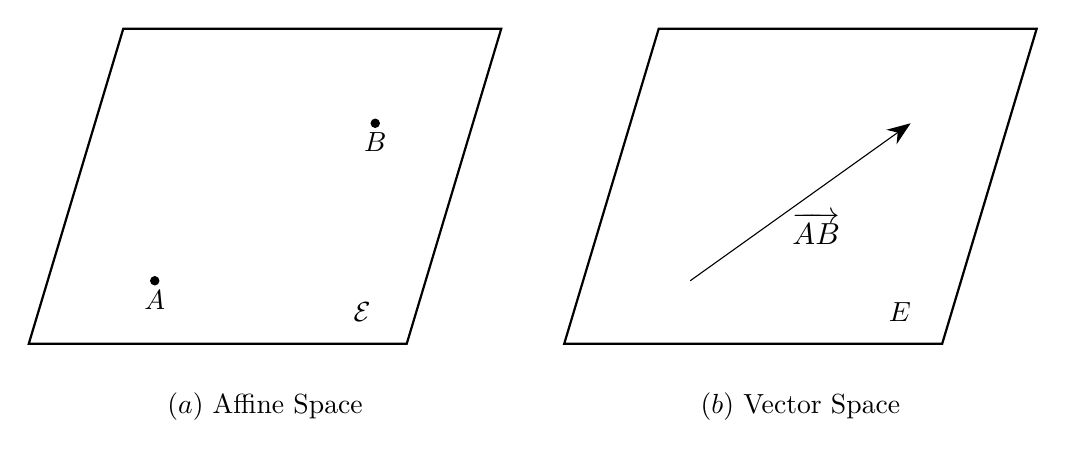
\begin{tikzpicture}[scale=4]
\usetikzlibrary {arrows.meta}
\usetikzlibrary {calc}

\begin{scope}[]
\draw[thick] (0, 0) -- (0.3, 1) -- (1.5, 1) -- (1.2, 0) -- cycle;
\fill[black] (0.4, 0.2) circle (0.015cm) node[below] {$A$};
\fill[black] (1.1, 0.7) circle (0.015cm) node[below] {$B$};
\node[right] at (1.0, 0.1) {$\mathcal{E}$};
\node[] at (0.75, -0.2) {($a$) Affine Space};
\end{scope}


\begin{scope}[shift={(1.7,0)}]
\draw[thick] (0, 0) -- (0.3, 1) -- (1.5, 1) -- (1.2, 0) -- cycle;
\draw[black, -{Stealth[length=3mm]}] (0.4, 0.2) -- (1.1, 0.7);
\node[below, scale=1.1] at (0.80, 0.45) {$\overrightarrow{AB}$}
;\node[right] at (1.0, 0.1) {$E$};
\node[] at (0.75, -0.2) {($b$) Vector Space};
\end{scope}
\end{tikzpicture}
\end{document}